% !TeX spellcheck = IT
\documentclass[12pt]{article}
\usepackage[top=1.5in, bottom=1.5in, left=1.2in, right=1.2in]{geometry}
\usepackage[utf8]{inputenc}
\usepackage[italian]{babel}
\usepackage{graphicx}
\usepackage{caption}
\usepackage[colorlinks=false,linkcolor=blue]{hyperref}
\usepackage{nameref} 
\usepackage{algorithm}
\usepackage[noend]{algpseudocode}
\graphicspath{{./images/}}
\def\code#1{\texttt{#1}}
\def\quote#1{``#1''}
\def\minquote#1{`#1'}
\def\image[#1][#2]#3{
  \begin{figure}[h]
  \centering
  \includegraphics[#2]{#1}
  \caption{#3}
  \end{figure}}
\def\boximage[#1][#2]#3{
	\begin{figure}[h]
		\centering
		\fbox{
		\includegraphics[#2]{#1}}
		\caption{#3}
\end{figure}}
\title{Il database sottostante Git}
\author{Arianna Masciolini}

\begin{document}
\maketitle
\newpage
\tableofcontents
\newpage
\section{Introduzione}
Git è un rinomato sistema di controllo versione distribuito che si appoggia ad un database non relazionale. L'importanza di tale database è tale da rendere una sua descrizione al giusto livello di approfondimento sufficiente per comprendere, con buona approssimazione, il funzionamento a basso livello di tale programma, spesso poco chiaro anche a chi lo utilizza quotidianamente. 
L'obiettivo di questo lavoro è appunto quello di aiutare l'utente di Git ad ottenerne un buon modello concettuale, utile per un uso più consapevole, e di spiegare quali vantaggi offra l'approccio adottato da Git nell'ambito della memorizzazione dei dati rispetto alle soluzioni adottate da gran parte dei sistemi concorrenti. 
\bigskip \\
Per raggiungere questo obiettivo, dopo alcuni cenni alla storia dei sistemi di controllo versione, i concetti fondamentali di Git verranno richiamati con una terminologia che dovrebbe risultare familiare ai suoi utenti, mentre la \hyperref[quarta sezione]{quarta sezione}, la più ampia, è dedicata specificamente al sottostante database, del quale mostra la struttura anche mediante alcuni esempi pratici, facendo uso di comandi poco noti, ma utili dal punto di vista didattico e sempre confrontati con i loro corrispettivi ad alto livello.
\section{Breve storia dei VCS}
Un \textit{Version Control System} (VCS) è un sistema che tiene traccia delle modifiche apportate ad uno o più file in modo da garantire all'utente la possibilità di accedere alle versioni precedenti dei file suddetti in qualsiasi momento. 
\bigskip \\
I primi sistemi di controllo di versione, locali, nacquero con l'idea di risolvere i problemi legati a quello che potrebbe essere definito versioning \quote{manuale}, consistente nel conservare più copie dei file d'interesse: la forte suscettibilità a errori e lo spreco di spazio su disco. Tra questi VCS locali, RCS ha goduto ha lungo di grande popolarità: esso salva su disco, in un particolare formato, una serie di \textit{patch}, ossia le differenze tra una versione e l'altra dei file, in modo tale da poter ricostruire lo stato in cui era ognuno di essi in qualsiasi momento, applicandovi una dopo l'altra le varie patch.
\bigskip \\
Successivamente, ci si pose il problema di permettere a più persone di collaborare a distanza. Per risolverlo nacquero i sistemi centralizzati di controllo di versione (CVCS), come CVS, Subversion, e Perforce. In questi sistemi, per il resto analoghi ad RCS e simili, tutte le versioni dei file controllati sono salvate su un unico server e rese così disponibili ai diversi utenti. Anche questo approccio presenta però problematiche importanti, dovute al fatto che il server centrale rappresenta un punto di vulnerabilità per l'intero sistema. 
\bigskip \\
I DVCS (\textit{Distributed VCS}), di cui Git, Mercurial, Bazaar e Darcs sono gli esempi più noti, risolvono questo problema: i membri del gruppo non si limitano a scaricare la più recente versione dei file, ma copiano l'intero repository, cosicchè ogni client costituisce un backup completo del progetto.
\begin{figure}[h]
	\centering
		\begin{minipage}{4cm}
			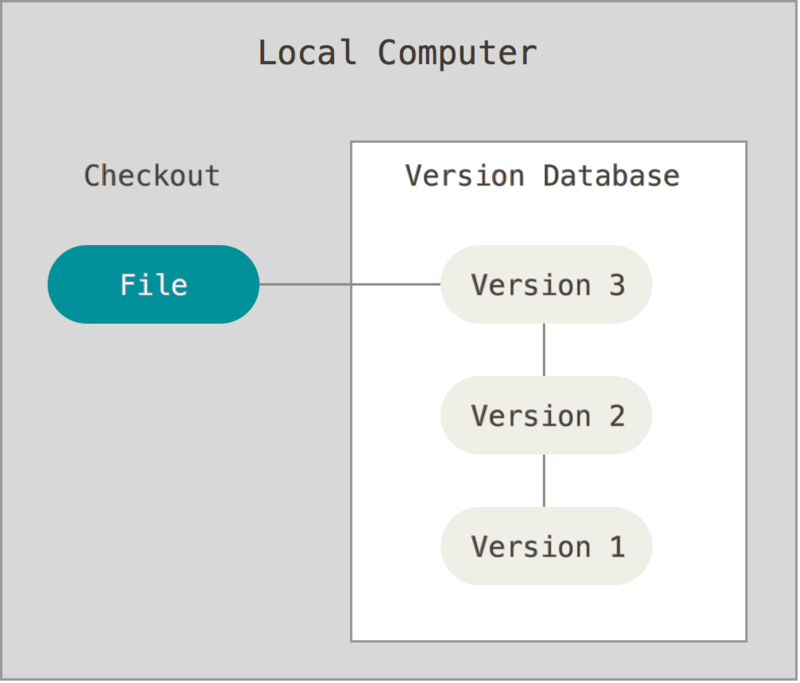
\includegraphics[height=3.5cm]{local.png}
		\end{minipage}
		\qquad
		\begin{minipage}{4cm}
			 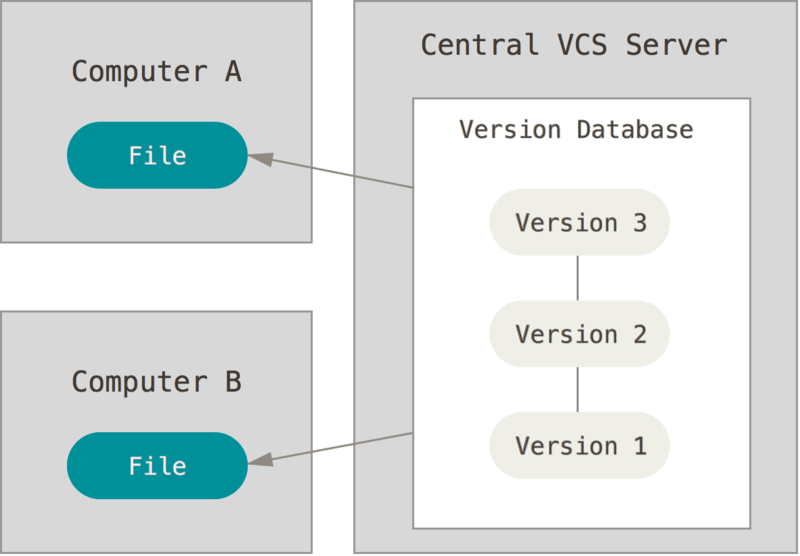
\includegraphics[height=3.5cm]{centralized.png}
		\end{minipage}
		\qquad
		\qquad
		\begin{minipage}{4cm}
			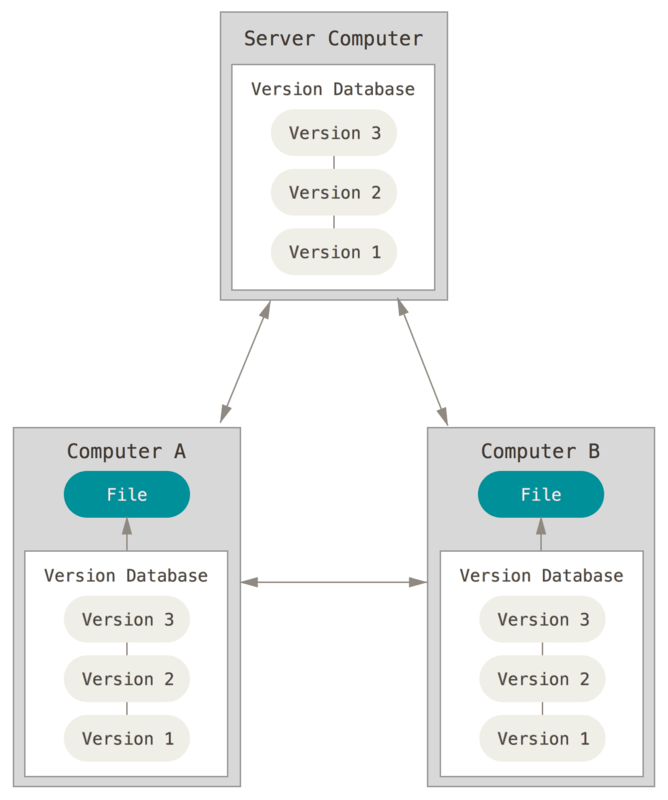
\includegraphics[height=3.5cm]{distributed.png}
		\end{minipage}
	\caption{Confronto tra un VCS locale, un CVCS e un DVCS.}
\end{figure}
\\In particolare, Git -ad oggi il VCS più diffuso \cite{openhub}- si differenzia tanto dagli altri sistemi distribuiti quanto dai loro predecessori per il modo in cui memorizza i dati: non come una serie di \textit{patch} legate ai vari file, ma come una serie di \quote{istantanee} di un filesystem in miniatura, accessibili tramite puntatori.
\section{Nozioni di base su Git}
Git, nato nel 2005 per favorire lo sviluppo del kernel Linux, è un sistema di controllo versione completamente distribuito che deve il suo successo al proprio modello di branching, che lo rende ottimale per la gestione di progetti open source, che hanno quasi sempre uno sviluppo non lineare.
\bigskip \\
Come si è accennato nella sezione precedente, Git adotta un approccio radicalmente differente rispetto a quello tradizionale, il cosiddetto controllo versione \textit{delta-based}, basato su una lista di \textit{patch}, ossia di modifiche, legate ai singoli file. Un repository Git è infatti una sorta di filesystem Unix-like semplificato, di cui viene fatta una sorta di \quote{istantanea} resa accessibile mediante un puntatore ogniqualvolta lo stato del progetto viene salvato.
\begin{figure}[h]
	\centering
	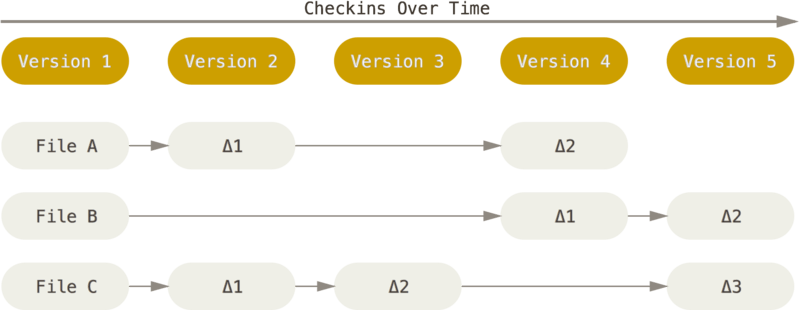
\includegraphics[width=13cm]{delta-based.png}
	\caption*{(a)\bigskip}
	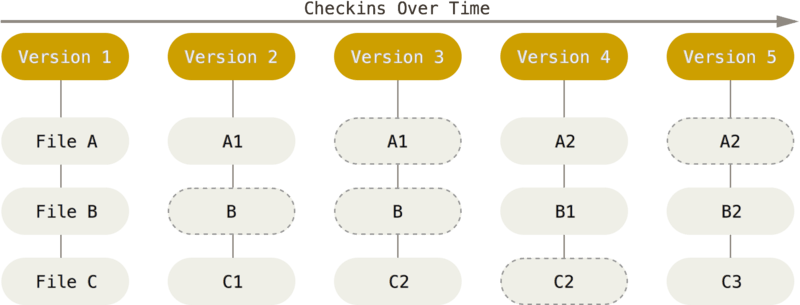
\includegraphics[width=13cm]{snapshots-based.png}
	\caption*{(b)}
	\caption{Confronto il modo in cui vengono salvati i dati in un VCS delta-based (a) e quanto avviene in Git (b).}
\end{figure}
\bigskip \\
Quasi tutte le azioni possibili in Git consistono, in ultima analisi, nell' \textit{aggiungere} dati al sottostante database. Cancellare dei dati e, in generale, compiere azioni distruttive, è reso volutamente difficile, in modo tale da rendere pressoché impossibile perdere il proprio lavoro, se non altro a seguito di un \textit{commit}, l'azione tramite la quale i cambiamenti al repository vengono salvati.
\bigskip \\
Per meglio comprendere quale sia il significato di un commit in Git e, in generale, per ottenere un buon modello concettuale del funzionamento di tale sistema di controllo versione, è fondamentale conoscere gli stati in cui può trovarsi un file all'interno di un repository:
\begin{itemize}
	\item \textit{modified}: sono state effettuate delle modifiche al file, non ancora confermate tramite un commit;
	\item \textit{staged}: il file, che ha subito delle modifiche, è stato marcato come parte del prossimo commit;
	\item \textit{committed}: il file è salvato permanentemente nel database locale tramite, appunto, un commit.
\end{itemize}
A questo punto è opportuno parlare della struttura di un repository Git, le cui parti principali sono:
\begin{itemize}
	\item il \textit{working tree}, consistente in una copia di una specifica versione del progetto, estratta dal database in modo da poter essere modificata dall'utente;
	\item la cartella \code{.git}, dove vengono si trovano i metadati e l'\textit{object database}, sui cui ci soffermerà nella prossima sezione, relativi al progetto;
	\item la \textit{staging area}, ossia il contenuto del prossimo commit, le informazioni relative al quale sono memorizzate nel file \code{index}, generalmente contenuto nella cartella \code{.git}. 
\end{itemize}
E' facile intuire, a questo punto, quale sia il tipico modo di procedere quando si lavora ad un progetto gestito con Git: dopo aver modificato uno o più file nel \textit{working tree}, si selezionano le modifiche di cui tener traccia nel commit successivo, aggiungendoli così alla \textit{staging area}. Nel momento in cui viene eseguito il comando \code{git commit} lo stato dei file nella \textit{staging area} viene salvato nella cartella \code{.git}.
\paragraph{Checksumming}
Un'ulteriore, importante funzionalità di Git, parte integrante della sua filosofia, è quella di verificare qualsiasi file o directory, prima di archiviarlo, tramite una checksum che è poi utilizzata per riferirvisi. Ciò significa che è impossibile cambiarne il contenuto senza che Git ne sia a conoscenza, il che permette di rilevare qualsiasi perdita o corruzione di dati in transito. 
Il meccanismo impiegato per generare tale checksum è la funzione crittografica SHA-1, il cui output, basato sul contenuto di un file o sulla struttura interna di una cartella, è un numero esadecimale di 40 caratteri.
\section{Il database di Git} \label{quarta sezione}% chapter: Git internals -> Git objects
La componente fondamentale di Git è un \textbf{database chiave-valore}: all'inserimento di un oggetto in un repository, Git restituirà una chiave, tramite la quale esso sarà univocamente identificato. 
Si può osservare in prima persona questo comportamento di Git utilizzando uno dei suoi comandi più a basso livello, \code{git hash-object}, che salva i dati che gli sono passati come input nell'\textit{object database}, ossia nella cartella \code{.git/objects}, e ne restituisce la checksum.
Inizializziamo dunque un nuovo repository, \code{demo}:
\begin{algorithm*}
	\begin{algorithmic}
		\State \code{\$ git init demo}
		\State \code{Initialized empty Git repository in /home/harisont/demo/.git/}	
	\end{algorithmic}
\end{algorithm*}
\\All'interno della cartella \code{.git} repository appena creato si trova, per l'appunto, la cartella dell'object database, contenente due sottocartelle, ma ancora nessun file\footnote{Il comando \code{find .git/objects -type f} serve a cercare tutti i file presenti nel repository.}:
\begin{algorithm*}
	\begin{algorithmic}
		\State \code{\$ cd demo}
		\State \code{\$ find .git/objects}	
		\State \code{.git/objects}	
		\State \code{.git/objects/info}
		\State \code{.git/objects/pack}
		\State \code{\$ find .git/objects -type f}
		\State \code{ \ }
	\end{algorithmic}
\end{algorithm*}
\bigskip \\Creiamo dunque un nuovo file vuoto ed inseriamolo nell'object database (senza l'opzione \code{-w}, ne otterremmo la checksum senza scrivere nulla nel database):
\begin{algorithm*}
	\begin{algorithmic}
		\State \code{\$ touch first}
		\State \code{\$ git hash-object first -w}	
		\State \code{e69de29bb2d1d6434b8b29ae775ad8c2e48c5391}	
	\end{algorithmic}
\end{algorithm*}
\bigskip \\
Chiaramente, a questo punto, la ricerca di file in \code{.git/objects} avrà un risultato di questo tipo:
\begin{algorithm*}
	\begin{algorithmic}
		\State \code{\$ find .git/objects -type f}
		\State \code{.git/objects/e6/9de29bb2d1d6434b8b29ae775ad8c2e48c5391}	
	\end{algorithmic}
\end{algorithm*}
\bigskip \\
Sono state create una sottocartella, il cui nome è costituito dai primi 2 caratteri della checksum, ed un file, ridenominato con i restanti 38.
A questo punto, abbiamo tutti gli strumenti per utilizzare, sia pure in modo molto semplice, il nostro sistema di controllo versione: facendo una modifica al file \code{first} e salvandola tramite \code{git hash-object}, si fa in modo che l'object database contenga entrambe le versioni del file, che resteranno disponibili anche qualora il file venisse rimosso dal \textit{working tree}:
\begin{algorithm*}
	\begin{algorithmic}
		\State \code{\$ echo \minquote{first modification!} > first}
		\State \code{\$ git hash-object first -w}	
		\State \code{\$ find .git/objects -type f}
		\State \code{.git/objects/e6/9de29bb2d1d6434b8b29ae775ad8c2e48c5391}
		\State \code{.git/objects/a9/16b860146f3db545e0e094f650d6e7b3dd4230}
	\end{algorithmic}
\end{algorithm*}
\ \\Tuttavia, utilizzare Git in questo modo è decisamente poco pratico, poiché per recuperare le versioni precedenti dei file è necessario utilizzare la checksum che lo identifica. Ciò è dovuto al fatto che, utilizzando il comando \code{git hash-object} non viene memorizzato il nome del file, ma solo il suo contenuto. Utilizzando la terminologia di Git, indicheremo gli oggetti di questo tipo come \textit{blob}.
\subsection{Tipi di oggetti in Git}
Chiaramente, i \textbf{blob} non sono i soli oggetti presenti in Git.
Per permettere di salvare i nomi dei file e di raggrupparli, Git utilizza anche oggetti di tipo \textit{\textbf{tree}}. 
Per meglio comprendere il ruolo che giocano questi due tipi di oggetti, basti pensare all'analogia tra Git ed un filesystem Unix: da una parte, i blob corrispondono, grosso modo, agli \textit{inodes}\footnote{in Unix, sono così chiamate le strutture dati che descrivono un oggetto del filesystem, ossia un file o una directory, memorizzandone i metadati e la posizione sul disco \cite{winode}.}, dall'altra i tree corrispondono alle directory. 
Un oggetto di tipo tree contiene un puntatore SHA-1 ad un blob o ad un sottoalbero.
\begin{figure}[h]
	\centering
	\begin{minipage}{7cm}
		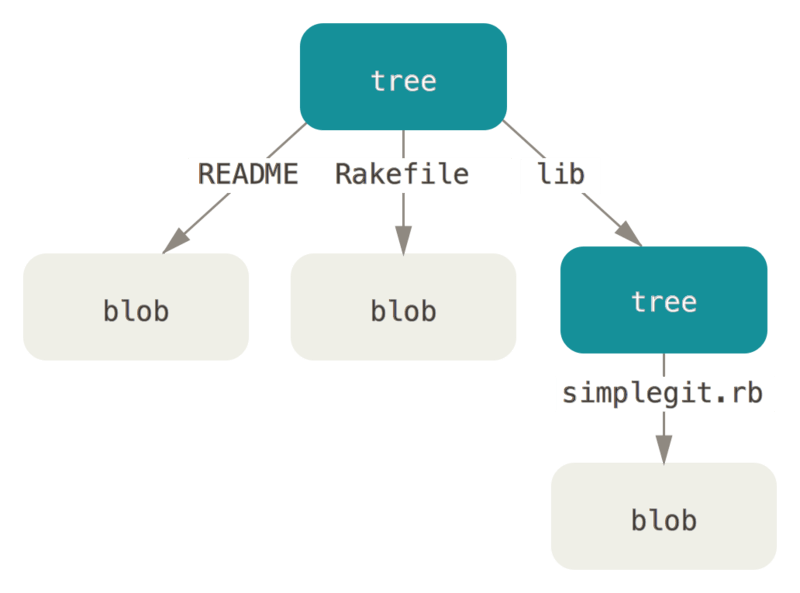
\includegraphics[height=5cm]{data-model-graph.png}
	\end{minipage}
	\qquad
	\begin{minipage}{7cm}
		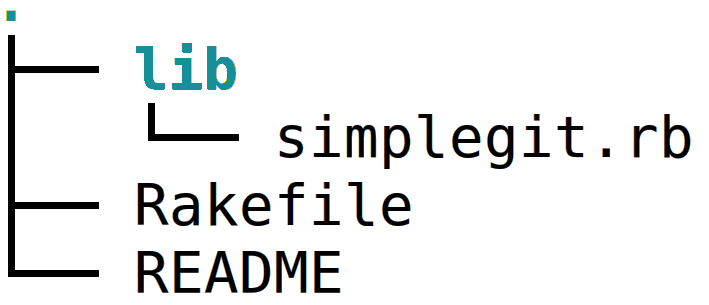
\includegraphics[height=2.5cm]{data-model-tree.png}
	\end{minipage}
	\caption{Corrispondenza tra oggetti di tipo tree e cartelle in un repository Git: sulla sinistra, il modello concettuale, sulla destra l'output del comando \code{tree}.}
\end{figure}
\bigskip \\
Poiché gli oggetti di tipo tree sono creati a partire dallo stato della staging area, cioè a partire dal file \code{index}, la creazione manuale di un oggetto di tale tipo richiede la creazione di un indice \textit{ad hoc}, per la quale si può utilizzare un altro comando a basso livello, \code{git update-index}, volto appunto ad aggiungere un file alla staging area, o il più noto \code{git add}, che aggiorna il file \code{index} con il contenuto del working tree \cite{git_ref}. Supponiamo di aver aggiunto alla staging area il file \code{README}: a questo punto, è possibile creare un oggetto tree, che sarà memorizzato nell'object database, tramite il comando \code{git write-tree}, che ne restituisce la checksum:
\begin{algorithm*}
	\begin{algorithmic}
		\State \code{\$ git write-tree}
		\State \code{543b9bebdc6bd5c4b22136034a95dd097a57d3dd}	
	\end{algorithmic}
\end{algorithm*}
\ \\Per verificare il tipo di un oggetto, si può fare uso del comando \code{git cat-file}, con l'opzione \code{-t}, mentre l'opzione \code{-p} serve a visualizzare il suo contenuto:
\begin{algorithm*}
	\begin{algorithmic}
		\State \code{\$ git cat-file -t 543b9bebdc6bd5c4b22136034a95dd097a57d3dd}
		\State \code{tree}
		\State \code{\$ git cat-file -p 543b9bebdc6bd5c4b22136034a95dd097a57d3dd}
		\State \code{100644 blob e69de29bb2d1d6434b8b29ae775ad8c2e48c5391 README}
	\end{algorithmic}
\end{algorithm*}
\ \\ 
Gli oggetti di tipo tree costituiscono, in pratica, la forma più semplice delle \quote{istantanee} di cui si è parlato nell'introduzione. Tuttavia, non risolvono tutti i problemi pratici del controllo versione: innanzitutto, con il solo uso di tree e blob, per recuperare le informazioni relative alle versioni precedenti di un progetto è necessario utilizzare le checksum, il che è poco agevole. Inoltre sarebbe utile salvare altre informazioni relative alle suddette \quote{istantanee}, come il loro autore, la data ed una descrizione. E' a questo proposito che sono stati introdotti gli oggetti di tipo \textit{\textbf{commit}}.
La creazione di un oggetto di questo tipo avviene tramite il comando \code{git commit-tree} - il corrispettivo a basso livello del più noto \code{git commit} - data la checksum di un tree, prendendo il messaggio di commit dallo standard input, restituisce l'id dell'oggetto creato:
\begin{algorithm*}
	\begin{algorithmic}
		\State \code{\$ echo 'first commit' | git commit-tree 543b9bebdc6bd5c4b22136034a95d\\ \ \ d097a57d3dd}
		\State \code{d03724c8f46342c5057107adc1c586feba5793ff}
	\end{algorithmic}
\end{algorithm*}
\ \\ 
La struttura di un commit è la seguente:
\begin{algorithm*}
	\begin{algorithmic}
		\State \code{\$ git cat-file -p d03724c8f46342c5057107adc1c586feba5793ff}
		\State \code{tree 543b9bebdc6bd5c4b22136034a95dd097a57d3dd}
		\State \code{author Arianna Masciolini <uzkamascio@gmail.com> 1531326893 +0200}
		\State \code{committer Arianna Masciolini <uzkamascio@gmail.com> 1531326893 +0200}
		\State 
		\State \code{first commit}
	\end{algorithmic}
\end{algorithm*}
\subsection{Memorizzazione degli oggetti}
In Git, ad ogni oggetto è associato un header che ne contiene il tipo, seguito da un spazio, dalla sua dimensione in byte e, per finire, da un byte nullo. La checksum dell'oggetto viene calcolata a partire dalla concatenazione dell'header con il contenuto stesso ed è in base a tale checksum, come accennato in precedenza, che viene stabilito il percorso in cui sarà salvato nell'object database: i primi due caratteri determinano la sottocartella, i restanti il nome del file.
\subsection{Riferimenti}
Il comando \code{git log}, data la checksum di un oggetto di tipo commit, permette di visualizzare lo storico dei commit di un repository a partire da quello specificato. Ad esempio, \code{git log d03724c8f46342c5057107adc1c586feba5793ff} restituisce:
\begin{algorithm*}
	\begin{algorithmic}
		\State \code{commit d03724c8f46342c5057107adc1c586feba5793ff}
		\State \code{Author: Arianna Masciolini <uzkamascio@gmail.com>}
		\State \code{Date:   Wed Jul 11 18:34:53 2018 +0200}
		\State 
		\State \code{first commit}
	\end{algorithmic}
\end{algorithm*}
\ \\
Anche in questo caso, l'uso della checksum risulta scomodo: è per questo che in Git sono presenti i riferimenti (\textit{refs}), una sorta di alias delle checksum SHA-1, salvate nella cartella \code{.git/refs}, che non contiene file, ma è strutturata come segue:
\begin{algorithm*}
	\begin{algorithmic}
		\State \code{\$ find .git/refs}
		\State \code{.git/refs}
		\State \code{.git/refs/heads}
		\State \code{.git/refs/tags}
	\end{algorithmic}
\end{algorithm*}
\ \\Un modo per creare un alias dell'ultimo commit, cui segue un esempio del suo utilizzo, è il seguente:
\begin{algorithm*}
	\begin{algorithmic}
		\State \code{\$ echo 1a410efbd13591db07496601ebc7a059dd55cfe9 > .git/refs/heads/\\ \ \ master}
		\State \code{\$ git log master}
		\State \code{commit d03724c8f46342c5057107adc1c586feba5793ff (HEAD -> master)}
		\State \code{Author: Arianna Masciolini <uzkamascio@gmail.com>}
		\State \code{Date:   Wed Jul 11 18:34:53 2018 +0200}
		\State
		\State \code{first commit}
	\end{algorithmic}
\end{algorithm*}
\ \\Se si vuole aggiornare un riferimento così creato, è consigliato non manipolarlo a mano, ma utilizzare il comando \code{git update-ref}\footnote{anche questo è un comando a basso livello, che raramente viene eseguito direttamente. Più spesso, si utilizza \code{git branch <branch>}, che tramite il comando \code{update-ref aggiunge la checksum dell'ultimo commit al ramo corrente.}}. 
E' così, in pratica, che funziona il branching di Git: un branch è infatti niente altro che un puntatore alla \code{HEAD}, un riferimento simbolico al ramo corrente, di una certa linea di sviluppo. 
\newpage
\begin{thebibliography}{9}
	\bibitem{git_pro}
	Scott Chacon, Ben Straub. \textit{Git Pro}, seconda edizione, 2014.
	\bibitem{git_ref}
	\href{https://git-scm.com/docs}{Git reference manual}. \\Ultima visita: 11/07/2018.
	\bibitem{openhub}
	\url{openhub.net}. \\Ultima visita: 5/7/2018.
	\bibitem{winode}
	Wikipedia. \href{https://en.wikipedia.org/wiki/Inode}{\textit{inode}}. \\Ultima visita: 10/7/2018.
	\bibitem{fun}
	Junio C. Hamano. \href{https://gitster.livejournal.com/39629.html}{\textit{Fun with updating the cached contents in the index by staging}}. \\Ultima visita: 11/07/2018.
\end{thebibliography}
\end{document}